% !TEX root = ../IS.tex
\chapter{Description of Software}
\section{AI Model}
To begin building an AI model, we first create a simulation of the game. The simulation has two players, each with 25 health points (HP). Both players have two possible actions per turn, which are randomly selected: attack the other player, reducing their opponents HP by 5 points, or heal themselves, increasing their HP by 4 points. Players can not heal above their starting value of 25 HP; any extra health points were discarded. Each action has a 50\% chance of occuring. The game runs until one player's HP was reduced to 0. The total number of turns and the sequence of actions are recorded into a CSV file. After running 4500 simulations, the data was imported into Matlab. A subset of the games are used as a training set for a decision tree, which predict which player would win the game.\\

\begin{figure}[H]
  \centering
  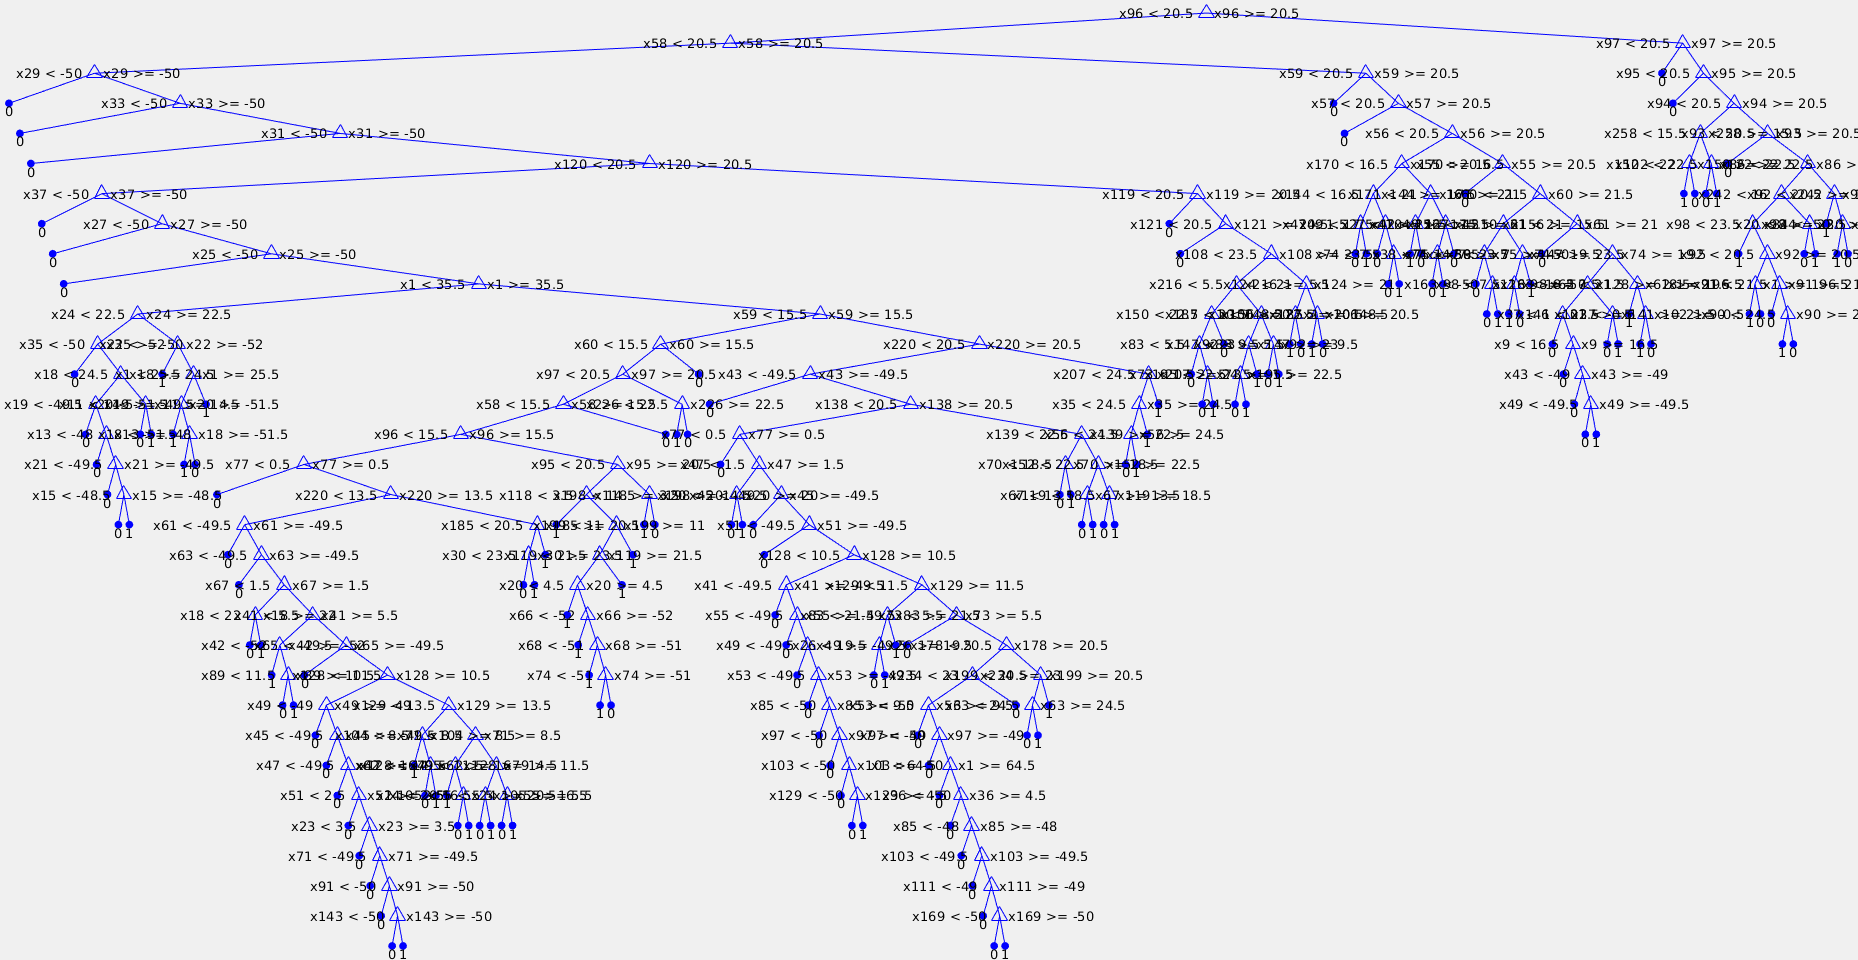
\includegraphics[width=13cm]{figures/firstDecisionTree.png}
  \caption{The decision tree generated from 4000 simulations of the game. This tree predicts 0 when player 1 wins and 1 when player 2 wins.}
  \label{fig:decisionTree1}
\end{figure}

However, this method is inconclusive, for a number of reasons. Firstly, the decision tree includes a large number of branches, as seen in Figure \ref{fig:decisionTree1}. Secondly, the actual criteria evaluated at each branch of the tree is different for each game. Aside from the first column, which contains the total number of turns in the game, and the second column, which contains the starting HP of player 1, the values in any particular column differ from game to game. For instance, the root node uses the value in column 96 as its classifier. In one game, column 96 may contain a HP value for player 2. In another, longer game, that column may contain a HP value for player 1. Thirdly, the individual games contain numerous streaks: a longer game is not the result of better strategy, but is instead caused by streaks where both players choose to heal on their turns. Players in these streaks reach HP levels near the 25 HP cap, effectively resetting the game.

The lack of consistency along columns is most likely the largest detriment to this model. Decision trees work best when classifying problems on specific attributes; if the attribute is different at column 96 from one game to another, the information gain at that column is meaningless. This is likely behind the sprawling nature of the decision tree itself. Without clear attributes to test, each split only has miniscule amounts of information gain.

A game theoretic angle is used on the second attempt. The HP of both players is reduced to 10, and two restrictions are added on healing: a player can not heal when they have full health, and a player can only heal themselves twice. With these new rules in place, we create an extensive-form tree for the new game.\\

\begin{figure}[H]
  \centering
  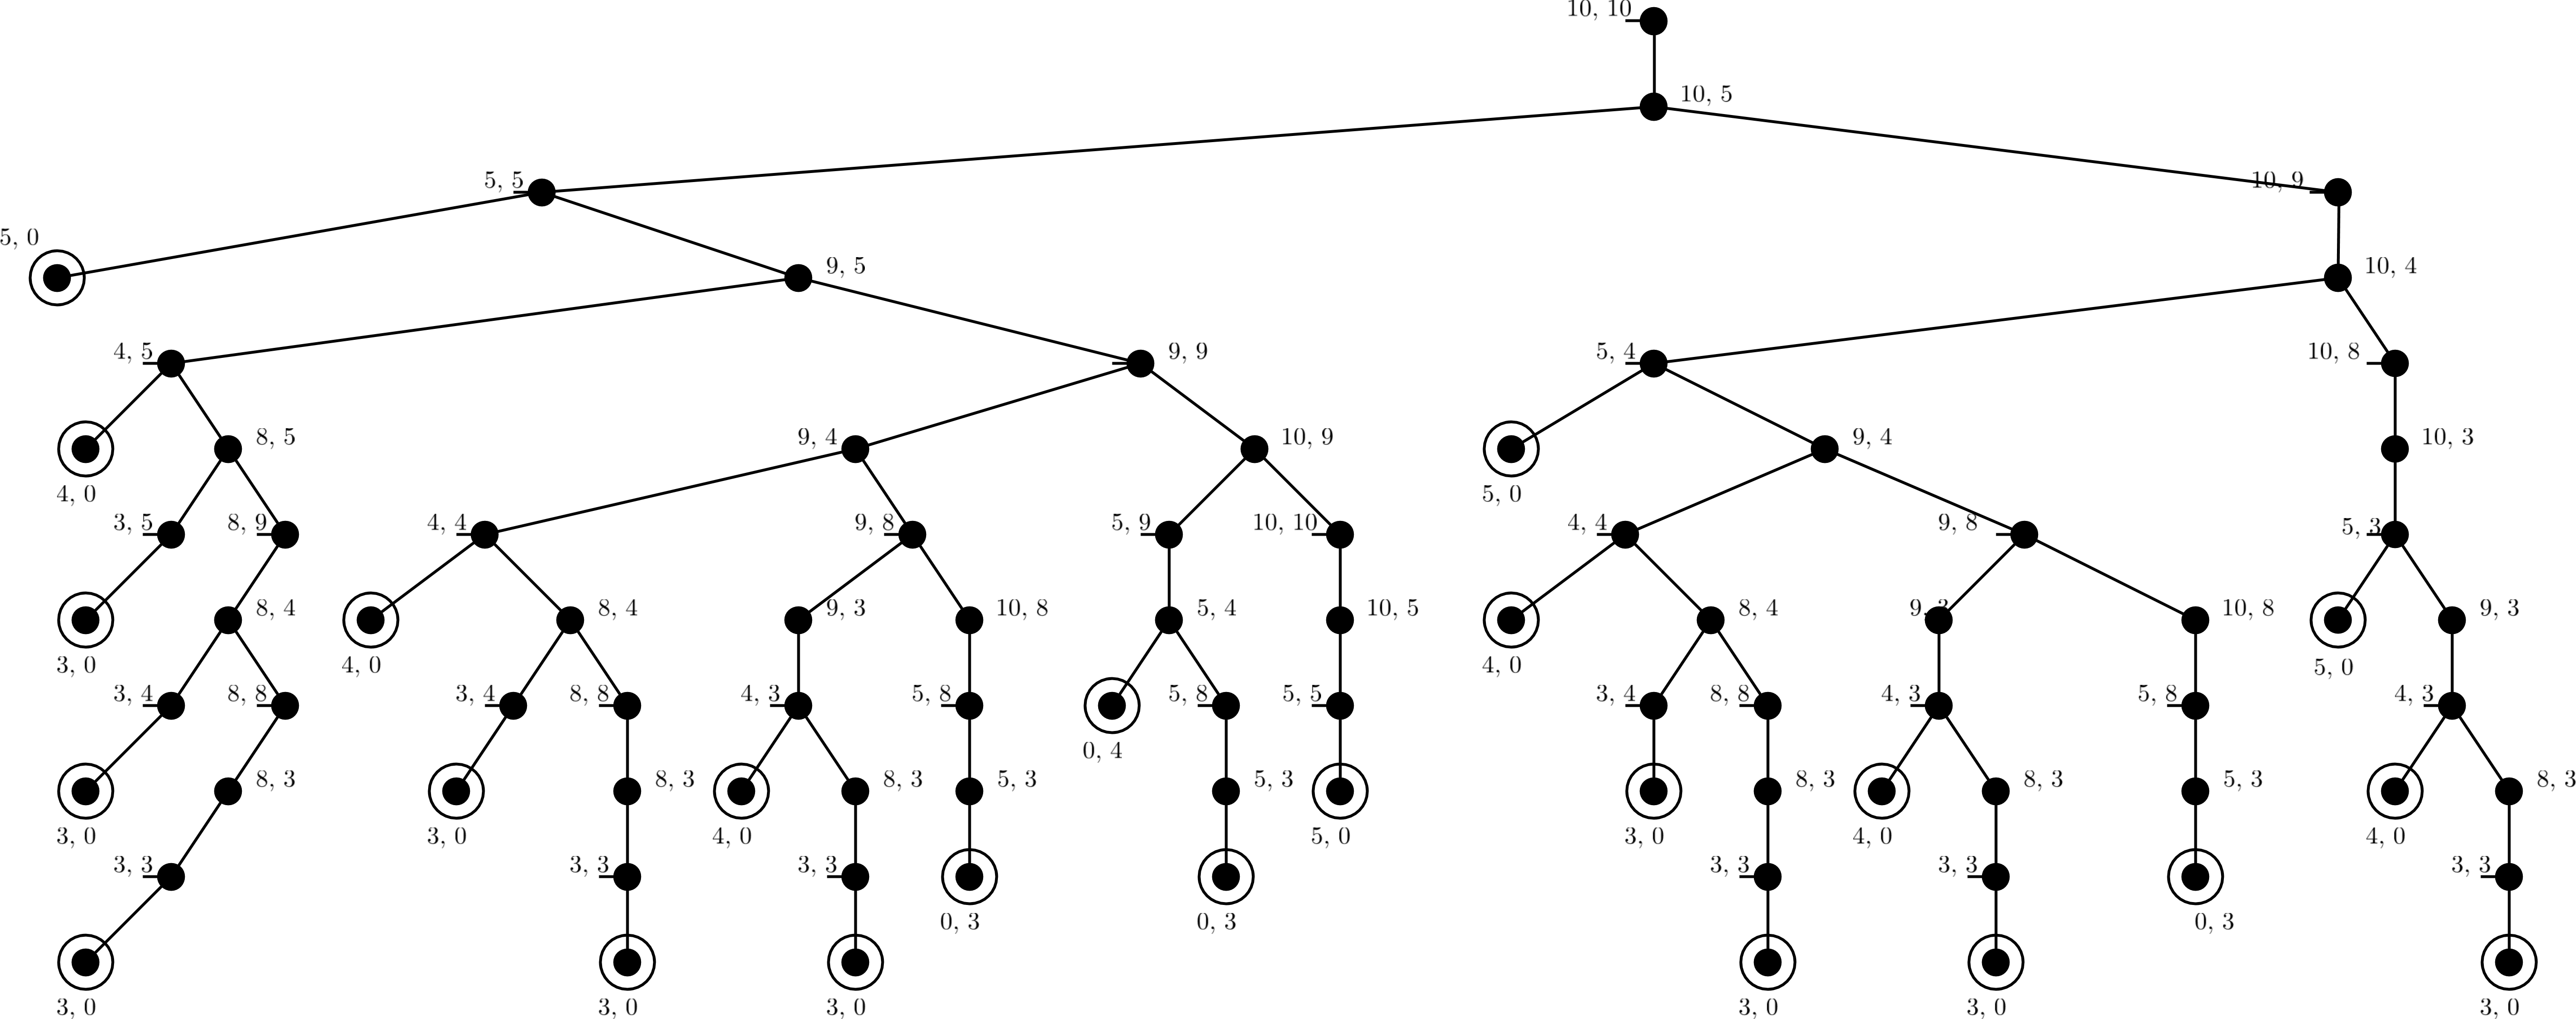
\includegraphics[width=15cm]{figures/GameTree.png}
  \caption{The extensive-form tree for a simplified game. Each player has 10 HP, and can only heal themselves twice.}
  \label{fig:gameTree}
\end{figure}

In Figure \ref{fig:gameTree}, player 1's nodes are denoted by a small dash to the left of the node. The HP values at each node are recorded, and leaf nodes are enclosed in a circle. There are 21 unique outcomes for this game; of these, only 4 of them result in a win for player 2, while the other 17 result in wins for player 1. In fact, with optimal play, player 1 will always win in this game.\\

\begin{figure}[H]
  \centering
  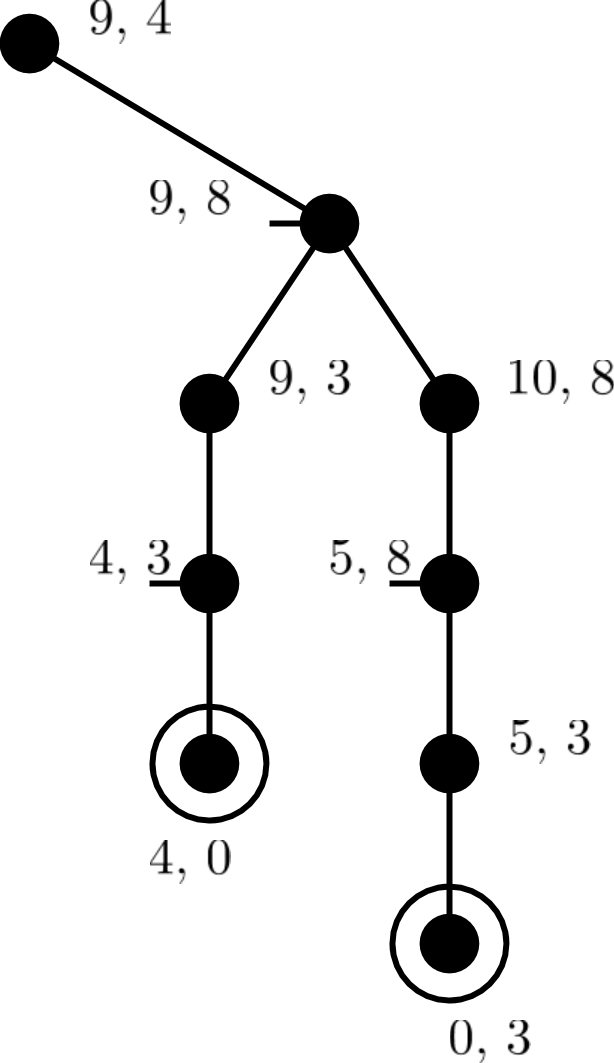
\includegraphics[width=4cm]{figures/GameSubtree.png}
  \caption{A subtree of the extensive-form representation}
  \label{fig:gameSubtree}
\end{figure}

For example, in this subtree, both player 1 and 2 have a winning outcome. However, the critical decision is made by player 1. Thus, in any game which reaches this subtree, player 1 will choose to attack on their turn, since that choice will lead to their victory.\\

\begin{figure}[H]
  \centering
  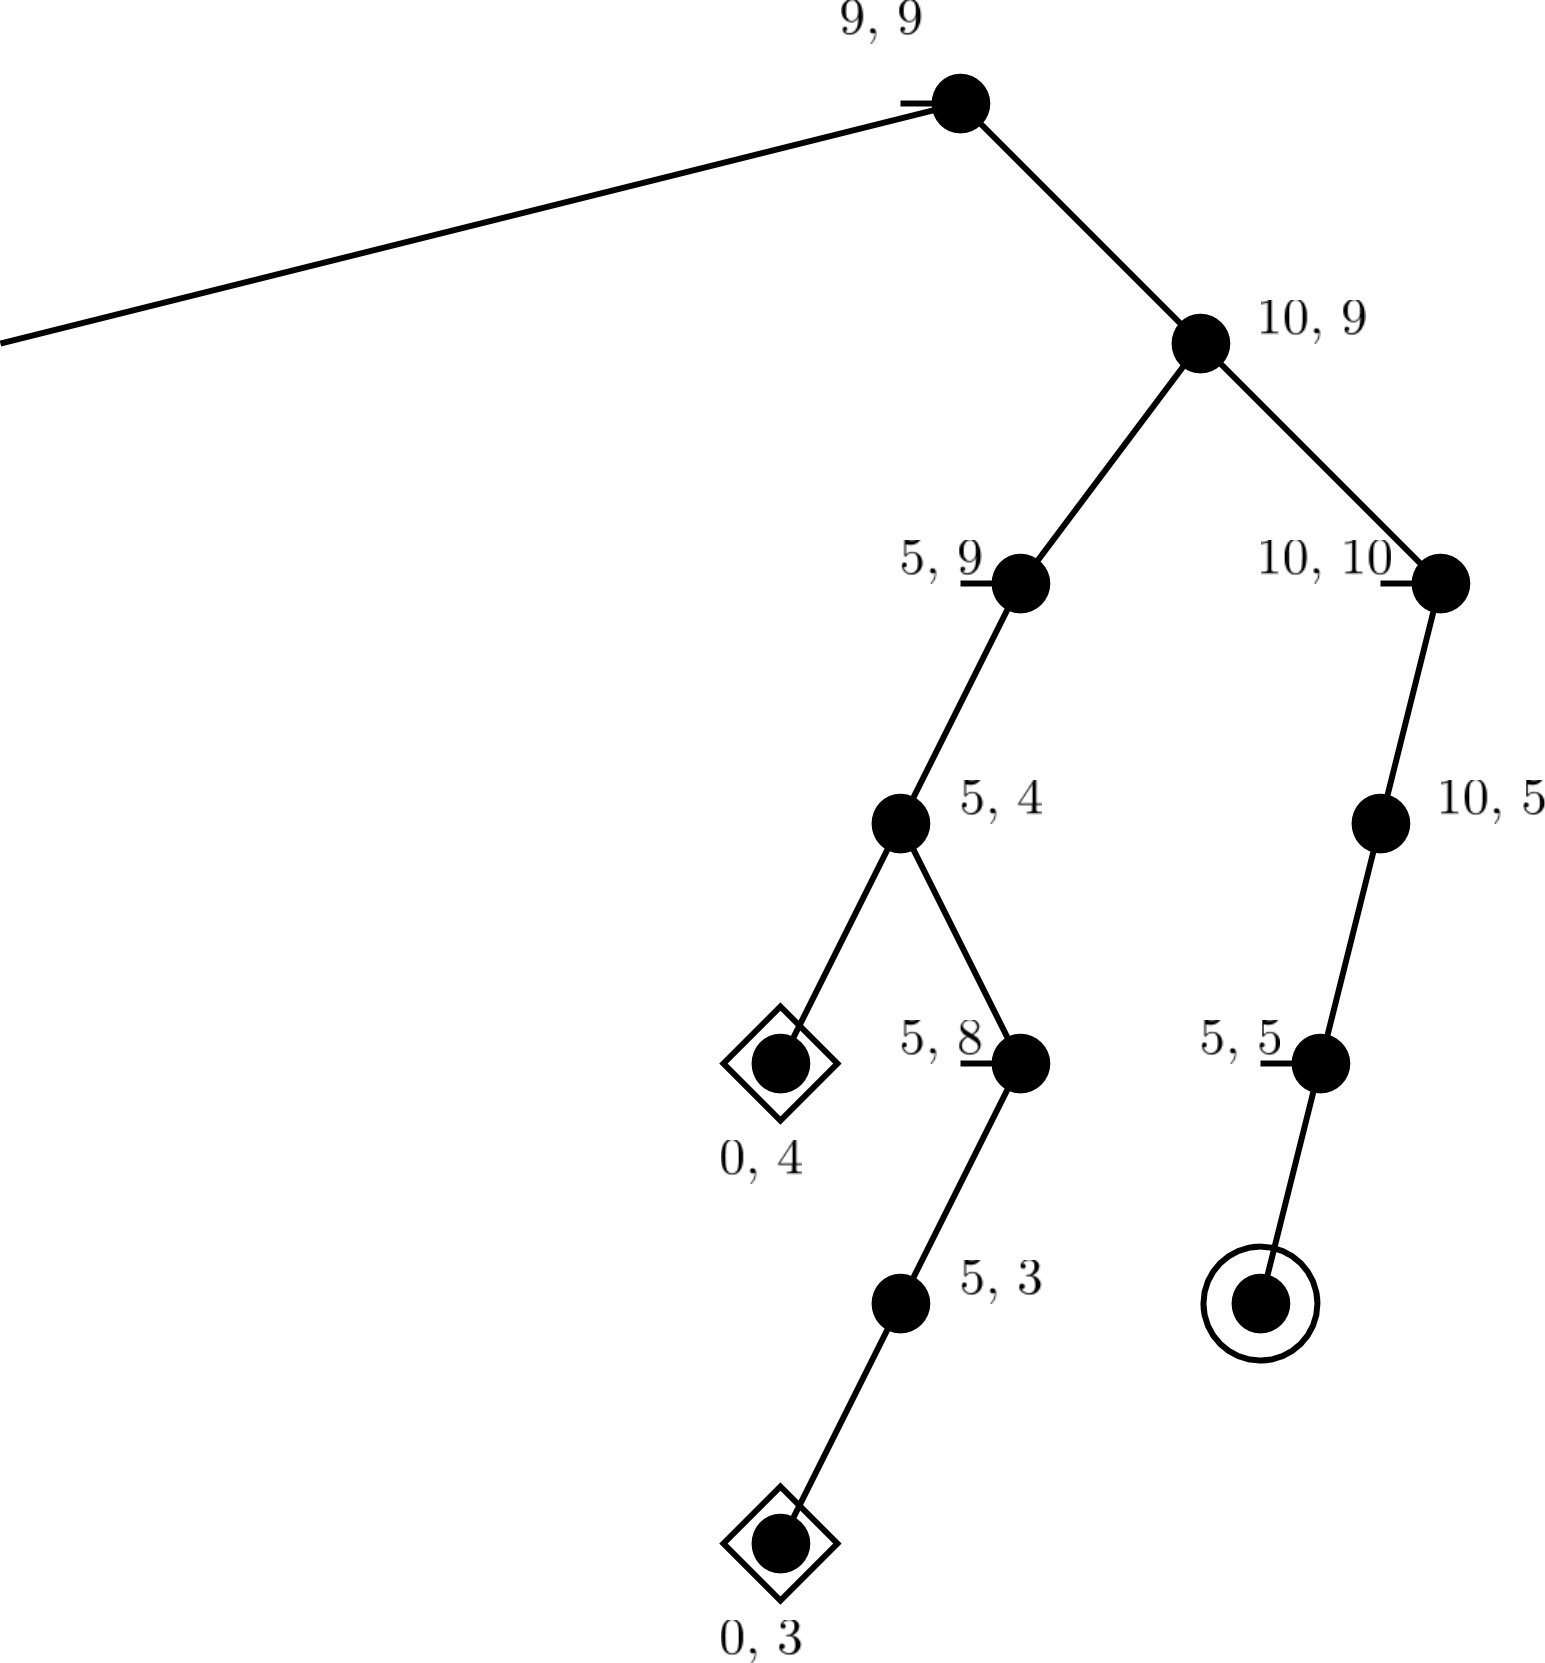
\includegraphics[width=7cm]{figures/GameSubtree2.png}
  \caption{A larger subtree of the extensive-form representation}
  \label{fig:gameSubtree2}
\end{figure}

The remainder of player 2's winning outcomes can be seen in the subtree in Figure \ref{fig:gameSubtree2}. At the root node of this subtree, player 1 is making their choice. If they choose to heal, the game moves into the right child. Player 2's first choice on the right child's subtree will either result in a win (if player 2 attacks) or a loss (if player 2 heals).

\section{Game Engine}
\subsection{The pygame Library}
The pygame library provides a number of Python functions that are useful in creating a two-dimensional video game. The library was originally created in 2001 to combine Python with SDL (Simple DirectMedia Layer), a library of multimedia controls written for C \cite{shinners}. pygame can utilize a variety of different graphics libraries, including OpenGL, DirectX, the Linux frame buffer, and an ASCII art backend \cite{shinners}. The pygame library is supported by numerous operating systems, and the core functions of pygame use highly optimized C or assembly code.\\

At the top level, pygame controls the initialization and exiting of its various modules, particularly the pygame.display module which renders the game. pygame features two functions to update a display window, pygame.display.flip() and pygame.display.update(). display.flip() works with two separate arrays, containing the pixel data for the window in which the game operates. One array is displayed by the screen, while the other array is used to record changes made to the on-screen image. Once all changes are made, display.flip() swaps these arrays, or ``buffers,'' by copying all the data from one array into the other. The buffer which recorded changes is now displayed on-screen, while the buffer that was displayed can now be used to record further changes. display.update() is an optimized version of flip() that takes as an argument a rectangle or a sequence of rectangles. These rectangles correspond to the areas of the display that need to be updated. For instance, passing the coordinates of a rectangle over a game's scoreboard will only update the scoreboard. With this function, large sections of the pixel array do not need to be copied from one buffer to another, speeding up the rendering process.\\

The two main objects in pygame are the Surface object and the sprite object. Surfaces can be changed with pygame to alter various attributes. For instance, the alpha value, or the transparency of the surface, can be changed with set\_alpha(). The individual color values can be converted to integers and vice versa with the map\_rgb() and unmap\_rgb() functions, respectively. This allows for pygame to store colors as a single number, rather than a tuple of integers. Surfaces are mostly used to load image files and to create backgrounds for the game. Sprites, on the other hand, are used for the actual in-game objects, such as enemies, player characters, and projectiles. Sprites can be stored in a Group object, which can be used to separate sprites by different purposes. Each sprite draws its image to a Surface, provided that it has a Surface.image and Surface.rect attribute.\\

Once a sprite or surface has been created with an image, pygame can also perform graphical transformations on that image. The pygame.transform module has functions to flip, rotate, and scale an image. Another Pygame feature is the ability to do collision detection on sprites and rectangles.\\

For the actual gameplay of a pygame program, there are also modules for joystick, mouse, and keyboard controls. A sound mixer module allows audio tracks to be played in the game, and the pygame.time module controls the framerate of the game.